\documentclass[twocolumn]{article}
\usepackage{graphicx}
\usepackage{listings}
\usepackage{booktabs}

\title{Math 308 Exercises 2.8}
\author{Nakul Joshi}

\renewcommand{\thesection}{}
\renewcommand{\thesubsection}{\alph{subsection})}
\newcommand{\includecode}[1]{\lstinputlisting{#1}}
\newcommand{\code}[1]{\lstinline{#1}}

\begin{document}
\lstset{language=R}
\graphicspath{ {./img/} }
\maketitle

\section*{2}
$
\overline{x}=6.5\\
m=5.5\\
\tilde{x}=2.389726\\
\tilde{m}=2.342779\\
f(\overline{x})\neq \tilde{x}\\
f(m)\neq \tilde{m}
$

\section*{4}

\subsection{}
\begin{table}[h]
\centering
    \begin{tabular}{ccccc}
    4-8am & 8-Noon & Noon-4pm & 4-8pm & 8-Mid \\
    699   & 1053   & 1048     & 972   & 257   \\
    \end{tabular}
\end{table}
\begin{figure}[h]
\centering
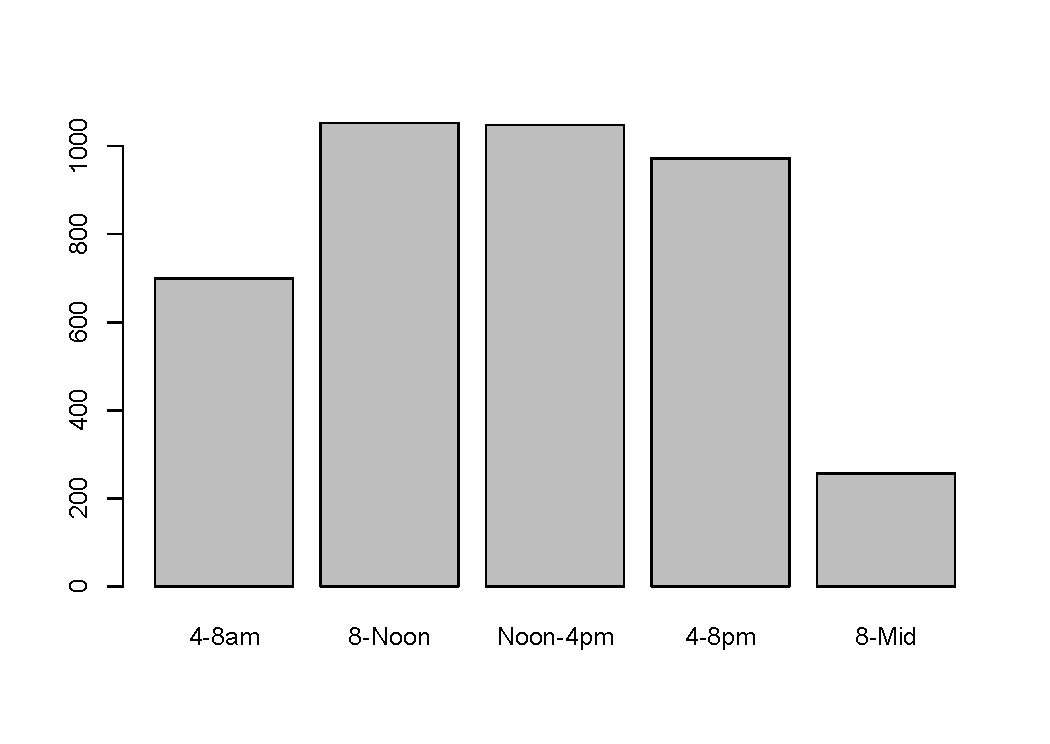
\includegraphics[width=0.4\textwidth]{4a.pdf}
\end{figure}
\newpage

\subsection{}
% Booktabs require to add \usepackage{booktabs} to your document preamble
\begin{table}[h]
\centering
\begin{tabular}{@{}lrrr@{}}
\toprule
  & No  & Yes & Proportion \\ \midrule
Mon & 569 & 61  & 0.09682540 \\
Tue & 535 & 93  & 0.14808917 \\
Wed & 488 & 76  & 0.13475177 \\
Thu & 434 & 132 & 0.23321555 \\
Fri & 493 & 144 & 0.22605965 \\
Sat & 406 & 47  & 0.10375276 \\
Sun & 507 & 44  & 0.07985481\\
\bottomrule
\end{tabular}
\end{table}
\end{document}